%%%%%%%%%%%%%%%%%%%%%%%%%%%%%%%%%%%%%%%%%%%%%%%%%%%%%%%
% LaTeX Template of MIST Thesis 
% Version 4.0 Date 31-03-2022
% Email: h.nyeem@eece.mist.ac.bd 
% -----------------------------------------------------
% This LaTeX template was originally developed by Lt Col Hussain Md Abu Nyeem, PhD, EME for the MSc Thesis students of the Military Institute of Science and Technology (MIST). The successive developments received updates with the specific policy and guidelines of MIST with a notable contribution of Major Md Abdul Wahed.
%
% This version quickly attempts for the first time to capture the prescribed format of the undergrad and postgrad theses of MIST students. This means that there would be surely some bugs and rooms for improvement.
%
% The main objective of this template is to facilitate the existing BSc/MSc/PhD Students of MIST to easily typeset their thesis content. This means that once the input-data of the title page are given, most of the sections of the front- and back-matters will be generated automatically.
%
% Please send us the email for further development of this template

%------------------------------------------------------
%HOW TO USE (A Brief Guideline for the Beginner)
%------------------------------------------------------
%1. Input the data for the front matters starting lines from: 119
%
%2. Images are to be copied in the FIGURE folder
%
%3. Update the Chapters in the CHAPTERS folder with the desired content
%
%4. Typesetting of abstract in Bengali is not yet supported by this version. However, a pre-typeset Bengali-abstract (written with avro in word or googledoc, and saved as pdf) can be included in the abstract section.
%
%5. Update the ACKNOWLEDGMENT, ABSTRACT, ABBREVIATIONS, SYMBOLS, ListOfPublication, and INDEX files in the CHAPTERS folder as well. Other pages of the front- and back-matters will be generated automatically.
%
%6. Reference files (bibtex files) are to be stored in the main directory where this file resides and the name of the bibtex file should be included in the \bibliography{FILENAME} in the REFERENCE section at the end of this document. Or, you may use/update the bibliographies in the current MyReference.bib file without further changes.


%%%%%%%%%%%%%%%%%%%%%%%%%%%%%%%%%%%%%%%%%%%%%%%%%%%%%%%
\pdfoptionpdfminorversion=5
%\RequirePackage{pdf14}
\RequirePackage{etex}
\makeatletter\let\MPtrue\@minipagetrue\makeatother

\documentclass[final,print]{packages/mistthesis}
\pdfminorversion=6

\makeatletter % disable the runtime redefinitions
\let\SS@makeulinesect\relax
\let\SS@makeulinepartchap\relax
\makeatother

%\usepackage{mathpazo}
\usepackage{notoccite}
\renewcommand{\bibname}{REFERENCES}

\usepackage[tight,footnotesize]{subfigure}
%\usepackage[caption=false]{subfig}

\usepackage{ragged2e}
%\usepackage[banglamainfont=Kalpurush, banglattfont=Siyam Rupali]{latexbangla}

%Table package
\usepackage{tabularx, threeparttable, longtable, float, multirow, array, pdflscape, afterpage, paralist}
\makeatletter
\def\true@true@true{\fi\fi\iftrue\iftrue\iftrue}
\makeatother

\usepackage{changepage, calc,  enumitem, linegoal, datetime}
\setlist[itemize]{itemsep=0cm}
\usepackage{booktabs, makecell}% http://ctan.org/pkg/booktabs
\newcommand{\tabitem}{~~\llap{\textbullet}~~}
\newlist{steps}{enumerate}{1}
\setlist[steps, 1]{label = \emph{Step} \arabic*:}

%using minipage environment in table
\makeatletter\let\MPtrue\@minipagetrue\makeatother
\newcommand{\figref}[2][{}]{\hyperref[#2]{\figurename~\ref{#2}#1}} 
\newcommand{\tabref}[2][{}]{\hyperref[#2]{\tablename~\ref{#2}#1}} 

\usepackage{hyphenat}
\def\hypp{--\penalty0\hskip0pt\relax}
\sloppy
\usepackage{emptypage, lscape, mdframed, rotating, afterpage}
\newcommand\blankpage{
	\null
	\thispagestyle{empty}
	\addtocounter{page}{-1}
	\newpage
}
\usepackage{listings}
\usepackage{etoolbox}
\makeatletter
\patchcmd{\@afterheading}%
{\clubpenalty \@M}{\clubpenalties 3 \@M \@M 0}{}{}
\patchcmd{\@afterheading}%
{\clubpenalty \@clubpenalty}{\clubpenalties 2 \@clubpenalty 0}{}{}
\makeatother
\appto\TPTnoteSettings{\footnotesize}
\AtBeginEnvironment{algorithmic}{\small}
% 
\makeatletter
\xpatchcmd{\algorithmic}{\itemsep\z@}{\itemsep=0.4ex plus1pt}{}{}
\makeatother
%
\makeatletter
\newcommand\fs@betterruled{%
	\def\@fs@cfont{\bfseries}\let\@fs@capt\floatc@ruled
	\def\@fs@pre{\vspace*{8pt}\hrule height.8pt depth0pt \kern2pt}%
	\def\@fs@post{\kern2pt\hrule\relax}%
	\def\@fs@mid{\kern2pt\hrule\kern2pt}%
	\let\@fs@iftopcapt\iftrue}
\floatstyle{betterruled}
\restylefloat{algorithm}
\makeatother
%\topskip=-20pt
\parskip=12pt
\parindent=0pt


%%%%%%%%%%%%%%%%%%%%%%%%%%%%%%%%%%%%%%%%%%%%%%%%%%%%%%%%%%%%%
%GIVE INPUT HERE FOR YOUR THESIS TITLE PAGE AND FRONT MATTERS
%%%%%%%%%%%%%%%%%%%%%%%%%%%%%%%%%%%%%%%%%%%%%%%%%%%%%%%%%%%%%
\makeatletter
% TITLE OF THE THESIS:
% Write the title in initial captial format 
% excluding that form for prepositions and conjuctions
\title{Title of My Thesis on a Topic of an Interesting Area of Engineering}
%% =========================================
%% Uncomment/Comment the Correct Thesis Type
%% =========================================
\ThesisType{B.Sc. Engineering Thesis}
% \ThesisType{M.Sc. Engineering Thesis}
%\ThesisType{Ph.D. Thesis}

%% =========================================
%% PG ONLY
%% Input F for full-timestudentship
%% Or, input P for part-time studentship
%% =========================================
%  \StudyType{F}


%===========================================================
%% NAMES & ROLL-NUMBERS OF THE STUDENTS AS AUTHORS:
%  For both the UG and PG students. 
%  Only First student is to be enabled for the PG Students.
%===========================================================
%% First student:
\FirstStudent{Student Name 1}  % Input the NAME of the first student
\FirstRoll{XXXXXXXXXX}  % Input the Student Number of the first student

%%Second student:
\SecondStudent{Student Name 2}  % Input the NAME of the second student, otherwise comment
\SecondRoll{XXXXXXXXXX}  % Input the Student Number of the second student, otherwise uncomment

%% Third student:
%\ThirdStudent{Student Name 3}  % Input the NAME of the second student, otherwise comment
%\ThirdRoll{XXXXXXXXXX}  % Input the Student Number of the second student, otherwise uncomment

%% Fourth student:
%\FourthStudent{Student Name 4}  % Input the NAME of the fourth student, otherwise uncomment
%\FourthRoll{XXXXXXXXXX}  % Input the Student Number of the fourth student, otherwise uncomment

%========================================================
%% ALL AUTHORS SUR NAMES FOR THE SPINE/SIDE OF HARD COVER
%========================================================
%   For multiple authors, include below all Surnames separated by \sep
%   For single author, only one surname is to be given without \sep
\AllSurNames{SURNAME1 \sep SURNAME2}

%=======================================
%% AUTHOR'S QUALIFICATION (FOR PG ONLY): 
%=======================================
%\qualifications{BSc Engg.\,(EEE), BUET} % For postgrad students only


%===================================================
% OTHER INFO (For all)
%===================================================
\session{20XX--20XX}
%
% DEGREE FOR THIS THESIS (No change for the BSc in EECE)
\degree{Bachelor of Science in Electrical, Electronic and Communication Engineering}

% LOGO OF MIST (NO CHANGE IS REQUIRED)
\logo{
\includegraphics[height=30mm, width=32mm]{logoMIST.png}}

% NAME OF THE DEPARTMENT AWARDING THE DEGREE 
%(NO NEED TO CHANGE FOR THE EECE DEPT STUDENTS)

\dept{Department of Electrical, Electronic and Communication Engineering}    % Input the full form of the dept

\deptShort{EECE} % Input the shaort form of the dept

% CITY OF THE UNIVERSITY (MIST): No change required
\MISTcity{Dhaka, Bangladesh}

% NAME OF THE UNIVERSITY (NO NEED TO CHANGE FOR THE MIST STUDENTS)
\university{Military Institute of Science and Technology}

% DATE OF THESIS DEFENSE
\DefenseDay{22}  % Day of the Defense
\DefenseDate{March 2022} % Month and Year of the Defense


%%%%%%%%%%%%%% SUPERVISOR AND EXAMINERS INFO %%%%%%%%%%%%
%% information of the supervisor
%% =============================
\SupervisorName{%
	Lieutenant Colonel Hussain Md. Abu Nyeem, PhD, EME}%
\SupervisorAffiliations{Instructor Class A}
\SupervisorInstitute{Department of EECE, MIST}
%
%% ===================================
%% information of the Head of the Dept
%% ===================================
\HeadName{Brigadier General A K M Nazrul Islam, PhD}%
\HeadAffiliations{Head of the Department}
\HeadInstitute{Department of EECE, MIST}
%======================================
%% Information of the Internal Member
%% ====================================
\InternalName{Md Golam Mostafa, PhD}%
\InternalAffiliations{Professor}
\InternalInstitute{Department of EECE, MIST}
%% =============================================================
%%  Uncomment the EXRTERNAL MEMBER BLOCK for the POSTGRAD thesis
%%  information of the External Member
%% =============================================================
% \ExternalName{Dr. Satya Prasad Majumder}%
% \ExternalAffiliations{Professor}
% \ExternalInstitute{Department of EEE, BUET}
% \ExternalCity{Dhaka\hypp 1205}


%%%%%%%% DO NOT EDIT THIS SECTION %%%%%%%%%%%%%%%%%%%%%%%%
%% =======================================================
%%%%%% DO NOT CHANGE the following block unknowingly %%%
%% =======================================================
% \ifdefined\@StudyType
% \author{\parbox{\textwidth}{\centering\@FirstStudent~(SN.~\@FirstRoll)}\fi}
% %\\SN.~\@FirstRoll (\@StudyType)}}%
% \else
% \makeatletter
\def\authorswithroll{\ifdefined\@FirstStudent
	\parbox{\textwidth}{\centering\@FirstStudent~(SN.~\@FirstRoll)}\fi\newline
	\ifdefined\@SecondStudent
	\parbox{\textwidth}{\centering\@SecondStudent~(SN.~\@SecondRoll)}\fi\newline
	\ifdefined\@ThirdStudent
	\parbox{\textwidth}{\centering\@ThirdStudent~(SN.~\@ThirdRoll)}\fi\newline
	\ifdefined\@FourthStudent
	\parbox{\textwidth}{\centering\@FourthStudent~(SN.~\@FourthRoll)}\fi}
	
	\def\onlyauthors{\ifdefined\@FirstStudent
	\parbox{\textwidth}{\centering\bf\@FirstStudent}\fi\newline
	\ifdefined\@SecondStudent
	\parbox{\textwidth}{\centering\bf\@SecondStudent}\fi\newline
	\ifdefined\@ThirdStudent
	\parbox{\textwidth}{\centering\bf\@ThirdStudent}\fi\newline
	\ifdefined\@FourthStudent
	\parbox{\textwidth}{\centering\bf\@FourthStudent}\fi}
    
    \author{\authorswithroll}
% \fi

%%%%%%%%%%%%%%%%%%%%%%%%%%%%%%%%%%%%%%%%%%%%%%%%%%%%%%%%%%
%%%%%% DO NOT EDIT UNKNOWINGLY: Setting up macros %%%%%%%%
%%%%%%%%%%%%%%%%%%%%%%%%%%%%%%%%%%%%%%%%%%%%%%%%%%%%%%%%%%
\let\thetitle\@title
\let\theauthor\@author
\let\theauthorswithroll\authorswithroll
\let\theonlyauthors\onlyauthors
\let\theThesisType\@ThesisType
\let\theStudyType\@StudyType
\let\thequal\@qualifications
\let\theroll\@roll
\let\thedegree\@degree
\let\thelogo\@logo
\let\thedept\@dept
\let\theuniversity\@university
\let\theMISTcity\@MISTcity
\let\thesubyear\@date
\let\thesession\@session
\let\theDefenseDay\@DefenseDay
\let\theDefenseDate\@DefenseDate
%-------------------------------------------------------
\ifdefined\@FirstStudent
\let\theFirstStudent\@FirstStudent
\let\theFirstRoll\@FirstRoll\fi
\ifdefined\@SecondStudent
\let\theSecondStudent\@SecondStudent
\let\theSecondRoll\@SecondRoll\fi
\ifdefined\@ThirdStudent
\let\theThirdStudent\@ThirdStudent
\let\theThirdRoll\@ThirdRoll\fi 
\ifdefined\@FourthStudent
\let\theFourthStudent\@FourthStudent
\let\theFourthRoll\@FourthRoll\fi 
%
\let\thesupervisor\@SupervisorName
\let\thesupervisorAffl\@SupervisorAffiliations
\let\thesupervisorUni\@SupervisorInstitute
%
\let\thehead\@HeadName
\let\theheadAffl\@HeadAffiliations
\let\theheadUni\@HeadInstitute
%
\let\theInternal\@InternalName
\let\theInternalAffl\@InternalAffiliations
\let\theInternalUni\@InternalInstitute
%
\let\theExternal\@ExternalName
\let\theExternalAffl\@ExternalAffiliations
\let\theExternalUni\@ExternalInstitute
\let\theExternalCity\@ExternalCity
\makeatother


%%%%%%%%%%%%%%%%%%%%%%%%%%%%%%%%%%%%%%%%%%%%%%%%%%%%%%%%%
%%%%%%%%%%%%%% YOUR DOCUMENT STARTS HERE %%%%%%%%%%%%%%%%
%%%%%%%%%%%%%%%%%%%%%%%%%%%%%%%%%%%%%%%%%%%%%%%%%%%%%%%%%
\begin{document}
	%\fontsize{11}{12.5}\rm 
	%\fontsize{11.5}{14}\rm
%	\setlength{\parindent}{0pt} 
%	\setlength{\parskip}{0.1\baselineskip}

	\makecover % Create the cover page for hard binding cover. It is not a part of your printed pages of the thesis.
	
	\makespine % Create the SPINE on the narrow binding side for hard binding cover. It is also not a part of your printed pages of the thesis.
	
	% \afterpage{\blankpage}
	\maketitle % This should be the first page of your thesis.
	

%% =======================================================
%%  Front Matter generates automatically that includes  	
%%  abstracts, approval certificate, ToC, Figure and 
%%  Table Lists etc.
%% =======================================================
	\frontmatter 
	
	
	%--------------------------------
	% Certificate of examiners
	% !TEX root = ../thesis.tex

\chapter*{APPROVAL CERTIFICATE}
%\chapter*{Approval Certificate}
%\addcontentsline{toc}{chapter}{APPROVAL CERTIFICSTE}

\parbox{\textwidth}{\centering\MakeUppercase{\thetitle}

\vspace{6pt}{\noindent\newline\theThesisType}

\vspace{6pt}By

\vspace{6pt}{\ifdefined\theStudyType\theauthor\else\authorswithroll\fi}
}

\noindent
{~~~Approved as to style and content by the %
\ifdefined\theStudyType Board of Examination on \theDefenseDay~\theDefenseDate\,:\else Examiners in \theDefenseDate\,:\fi
}


%\section*{Board of Examiners}
\vspace{\ifdefined\theStudyType 4ex \else 8ex\fi}


\begin{table*}[!h]
\resizebox{\textwidth}{!}{
		\begin{tabular}{llr}
		\makebox[70mm]{\hrulefill}& \hspace{1.5cm} &\\
		  %\cline{2-2}\\
		\thesupervisor &  \hspace{1.5cm} &Chairman \\
		\thesupervisorAffl & \hspace{1.5cm} &(Supervisor)\\
		\thesupervisorUni,~\theMISTcity &  \hspace{1.5cm} &\ifdefined\theStudyType Board of Examination\fi\\
			\vspace{\ifdefined\theStudyType 4ex \else 8ex\fi}\\
%
%
\ifdefined\theStudyType%
		\makebox[70mm]{\hrulefill}& \hspace{1.5cm} &\\
		%\cline{2-2}\\
		 \theInternal &  \hspace{1.5cm} &Member\\
		 \theInternalAffl & \hspace{1.5cm} &(Internal)\\
		 \theInternalUni,~\theMISTcity &  \hspace{1.5cm} &\ifdefined\theStudyType Board of Examination\fi\\
		\vspace{4ex}\\
		\fi
%
%
		\makebox[70mm]{\hrulefill}& \hspace{1.5cm} &\\
		%\cline{2-2}\\
		 \thehead   &  \hspace{1.5cm} &Member\\
		\theheadAffl & \hspace{1.5cm} &(Ex-officio)\\
		 \theheadUni,~\theMISTcity &  \hspace{1.5cm} &\ifdefined\theStudyType Board of Examination\fi\\
		\vspace{\ifdefined\theStudyType 4ex \else 8ex\fi}\\
		%	
%
\ifdefined\theStudyType%
		\makebox[70mm]{\hrulefill}& \hspace{1.5cm} &\\
		  %\cline{2-2}\\
			\theExternal   &  \hspace{1.5cm} &Member\\
			\theExternalAffl & \hspace{1.5cm} &(External)\\
			\theExternalUni,~\theExternalCity &  \hspace{1.5cm} &\ifdefined\theStudyType Board of Examination\fi\\\fi
% 
		\end{tabular}
		}
\end{table*}


\vfill
{\parbox{\textwidth}{\centering\quad\thedept\newline MIST, Dhaka}
%
%2. $---------------------------$ \hfill Member\\
%\quad Gp Capt Md Hossam-E-Haider, PhD, BAF \hfill (Ex-officio)\\
%\quad Professor and Head\\
%\quad Dept. of EECE, MIST, Dhaka - 1216

%\end{dedication}
	%\addcontentsline{toc}{chapter}{APPROVAL CERTIFICATE}
	%\listofalgorithms
	%--------------------------------
	
	%--------------------------------
	% Statement of Original Authorship
	%\statementofauthorship
	\chapter*{\normalfont\MakeUppercase\thetitle}
% \addcontentsline{toc}{chapter}{DECLARATION}
%\chapter*{Candidate's Declaration}
%\subsection*{}

% \vspace{18pt}
% \parbox{\textwidth}{\centering\MakeUppercase{\thetitle}}\\[14pt]
\parbox{\textwidth}{\centering\MakeUppercase{Declaration}}\\[14pt]

% \chapter*{DECLARATION}
%
% \vspace{18pt}
% \MakeUppercase{DECLARATION}}\\[18pt]

\noindent\ifdefined\theStudyType I \else We~\fi
hereby declare that the study reported in this thesis entitled as above is 
\ifdefined\theStudyType my \else our \fi
own original work and has not been 
submitted before anywhere for any degree or other purposes. Further,
\ifdefined\theStudyType I \else we \fi
certify that the intellectual content of this thesis is the product of 
\ifdefined\theStudyType my \else our \fi own work and that all the assistance received in preparing this thesis and sources have been acknowledged and cited in the reference section.


\vspace{10ex}


\begin{table*}[!h]
%	\resizebox{\textwidth}{!}{\small
	\noindent
		\begin{tabular}{l}
			\makebox[70mm]{\hrulefill}\\
				%\cline{2-2}\\
				\theFirstStudent \\
				\ifdefined\theStudyType 	\vspace{4ex}
				\else
					Student No. \theFirstRoll\\
					\vspace{6ex}\\
				%
				\ifdefined\theSecondStudent 
				\makebox[70mm]{\hrulefill}\\
				\theSecondStudent\\
				Student No. \theSecondRoll\\
				\vspace{6ex}\\\fi
				%
				\ifdefined\theThirdStudent 
				\makebox[70mm]{\hrulefill}\\
				\theThirdStudent\\
				Student No. \theThirdRoll\\
				\vspace{6ex}\\\fi
				%
				\ifdefined\theFourthStudent 
				\makebox[70mm]{\hrulefill}\\
				\theFourthStudent\\
				Student No. \theFourthRoll\\
				\vspace{6ex}\\\fi
				\fi\\
			%
%			%
%			\makebox[70mm]{\hrulefill}\\
%			%\cline{2-2}\\
%			\theInternal\\
%			\theInternalAffl\\
%			\theInternalUni\\
%			\vspace{5ex}\\
%			%
%			%
%			\makebox[70mm]{\hrulefill}\\
%			%\cline{2-2}\\
%			\thehead   \\
%			\theheadAffl\\
%			\theheadUni\\
%			\vspace{5ex}\\
%			%	
%			%
%			\ifdefined\theStudyType%
%			{\makebox[70mm]{\hrulefill}\\
%				%\cline{2-2}\\
%				\theExternal \\
%				\theExternalAffl\\
%				\theExternal\\}\fi
%			%
%			%
		\end{tabular}
%	}
\end{table*}

\vfill
{\parbox{\textwidth}{\centering\quad\thedept\newline MIST, Dhaka}

 


	%\addcontentsline{toc}{chapter}{CANDIDATE'S DECLARATION}
	%--------------------------------
	
	%--------------------------------
	% Dedication
	\ifdefined\theStudyType
	\chapter*{\normalfont\MakeUppercase\thetitle}
% \addcontentsline{toc}{chapter}{DECLARATION}
%\chapter*{Candidate's Declaration}
%\subsection*{}

% \vspace{18pt}
% \parbox{\textwidth}{\centering\MakeUppercase{\thetitle}}\\[14pt]
\parbox{\textwidth}{\centering\MakeUppercase{Dedication}

\vspace{15pt}{\noindent\newline A Thesis}

\vspace{8pt}By

\vspace{8pt}{\ifdefined\theStudyType\theFirstStudent\fi}
}

\vspace{5ex}
{\parbox{\textwidth}{\large\centering Dedicated to my parents for supporting and encouraging \\me to believe in myself.}}\fi
	%--------------------------------
	
		%--------------------------------
	% Acknowledgements
	% !TEX root = ../thesis.tex

\chapter*{ACKNOWLEDGEMENTS}

Foremost, I would like to express my sincere gratitude to my supervisor, \thesupervisor\ of the~\thesupervisorUni\ for the useful comments, remarks and engagement through the learning process of this master thesis. 
I always received appropriate guidelines, ....


I would also like to thank ....
%
I would also like to extend my heartfelt gratitude to  ....
%
I also thank the ....


Finally, I must express my profound gratitude to ....


%\vspace{1.25cm}
%\noindent
%{\hfill {\sc \theauthor}
%
%\smallskip
%\hfill {\it \theuniversity}
%
%\hfill {\it Dhaka, Bangladesh}
%
%\hfill {\it \theDefenseDate}}
%%\hfill {\it \monthname~2018}}


 






\vfill
%\end{acknowledgements}

	%--------------------------------
	
	
	% Abstract
	% !TEX root = ../thesis.tex

\begin{abstract}
	
\parbox{\textwidth}{\centering\large\bf\thetitle}\\[10pt]
	
\noindent%
Write the abstract of your work as an independent part of your thesis capturing the research problem and its significance, your contributions and its validation, and conclusions.
\looseness -1

\end{abstract}


	%
	\addcontentsline{toc}{chapter}{ABSTRACT (BENGALI)}
	% !TEX root = ../thesis.tex
\thispagestyle{plain}
%	\noindent%
%	Write the abstract of your work as an independent part of your thesis capturing the research problem and its significance, your contributions and its validation, and conclusions.
%	\looseness -1

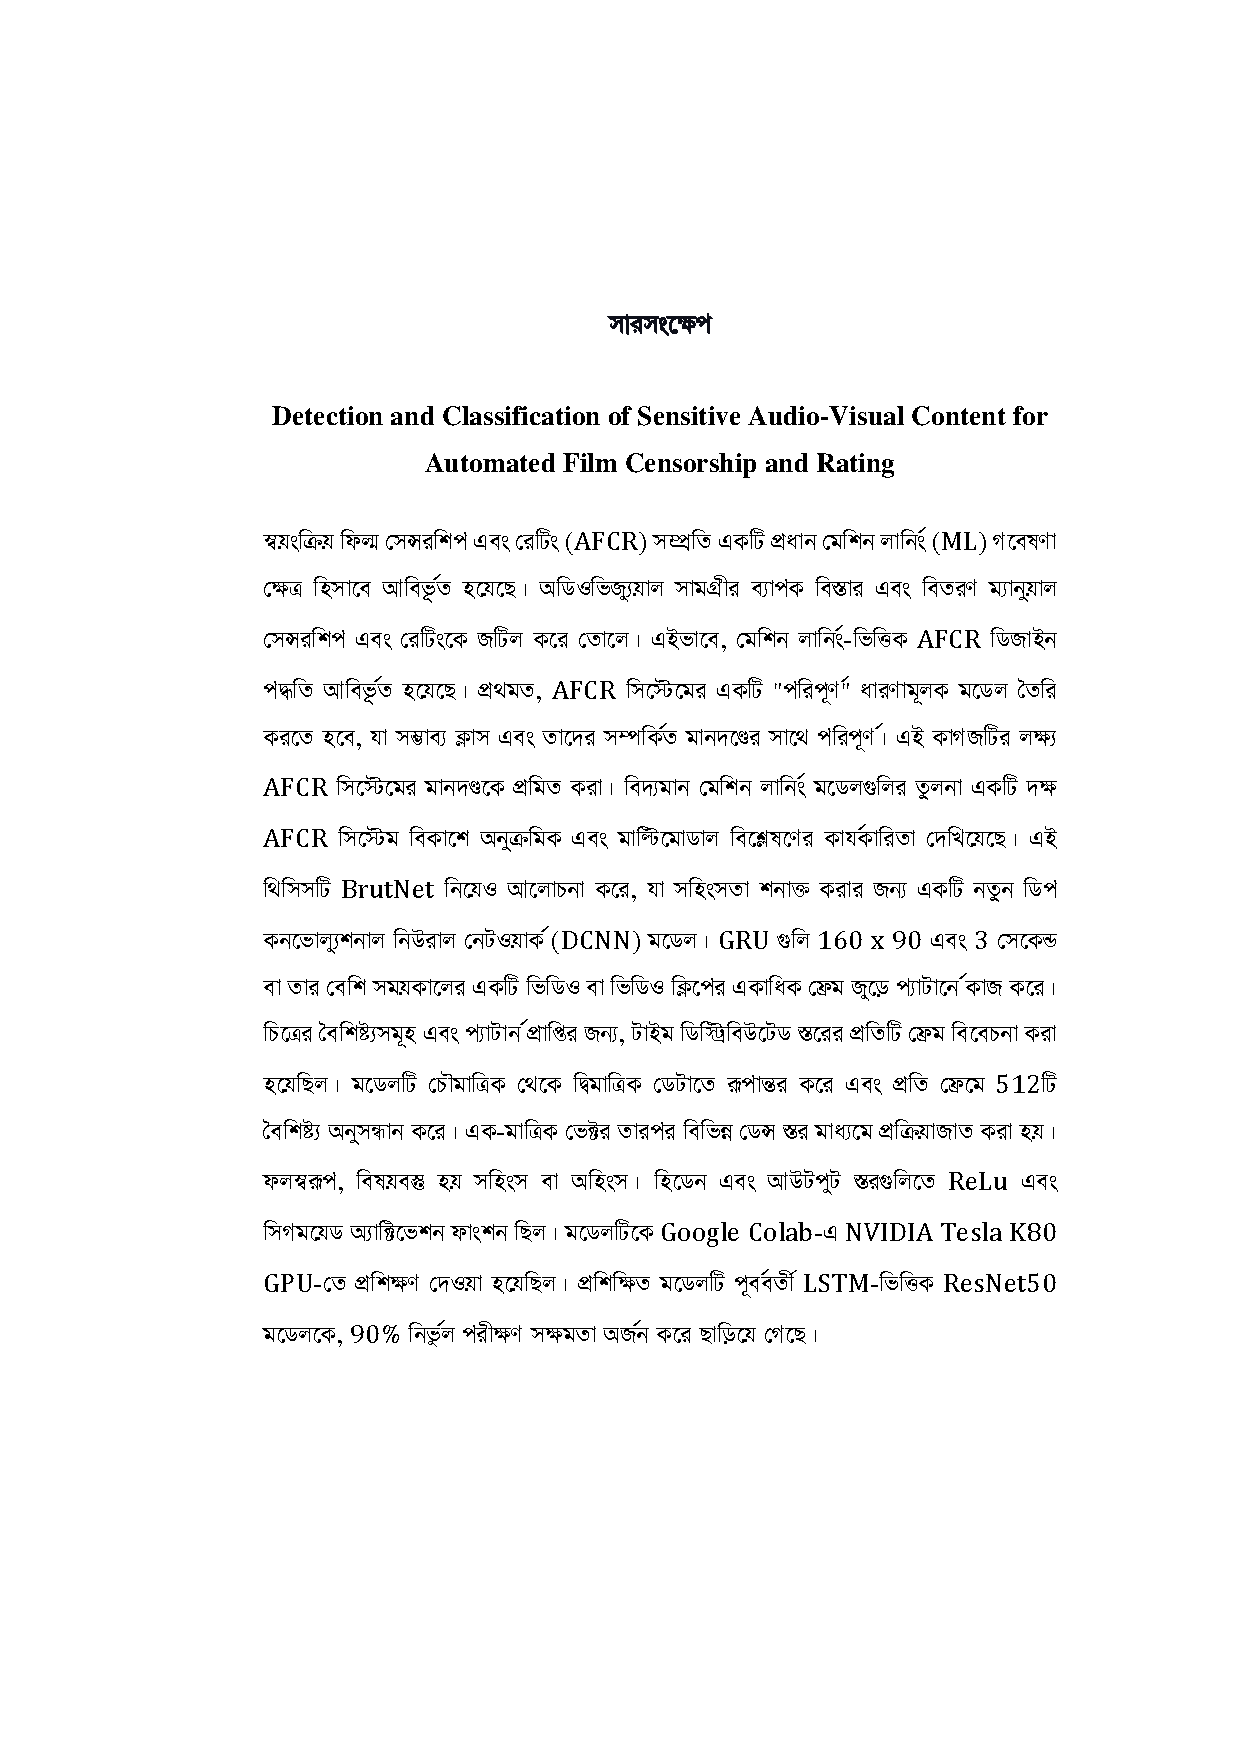
\includegraphics[width=\textwidth, keepaspectratio]{chapters/Benglali-abstract.pdf}
%\includepdf[pages={1,3,5-7}]{Bangla-abstract.pdf}

	
	%--------------------------------
	
	% List of SYmbols/Notations
	%--------------------------------
	%list of Symbols
\chapter{LIST OF NOTATIONS}
%\chapter{listofsymbols}
\noindent
\begin{longtable}[l]{p{60pt}p{300pt}}

$I$ 	       &   An input image \\
$\hat{I}$      &   An embedded version of the input image, $I$ \\ 
$M$ 	       &   Number of pixels in a row: $M \in \mathbb{N}$\\
$N$ 	 	   &   Number of pixels in a column: $N \in \mathbb{N}$ \\
NEW & ADD MORE, ADD YOURS\\
\end{longtable}

%\end{listofsymbols}

	%\addcontentsline{toc}{chapter}{List of Symbols}
	%\addcontentsline{toc}{chapter}{List of Abbreviations}
	%--------------------------------
	%--------------------------------
	% List of Abbreviations
	%--------------------------------
	\ifdefined\theStudyType
	%list of abbreviations


%\chapter{listofabbreviations}
\chapter{LIST OF ABBREVIATIONS}
\noindent

%comment the lines below
%List all the alphabetically sorted abbreviations with the following latex command in the long table environment: 

%%Uncomment the below table environment to enter abbreviations.
%%--------------------------------------
%\begin{longtable}[l]{p{55pt}p{300pt}}
%%%\textbf{LSB}		&	Least Significant Bit\\
%%%\textbf{MSB}		&	Most Significant Bit\\
%\end{longtable}

%\end{listofabbreviations}

	\fi
	%\addcontentsline{toc}{chapter}{List of Abbreviations}
%	%--------------------------------
	%-------------------------------------
	\renewcommand\listtablename{LIST OF TABLES}
	\listoftables
	%--------------------------------------
	%% List of Tables and Figures
	\renewcommand\listfigurename{LIST OF FIGURES}
	\listoffigures
	%%--------------------------------------
	% Table of Contents
	\tableofcontents
	%--------------------------------
	
	%--------------------------------------
	
	%\renewcommand\listalgorithmname{LIST OF ALGORITHMS}  
	%\let\oldlistofalgorithms\listofalgorithms
	%\captionsetup[algorithm]{labelsep=colon}
	%\makeatletter
	%\renewcommand{\listofalgorithms}{%
	%\begingroup%
	%\let\oldnumberline\numberline%
	%\let\old@dottedtocline\@dottedtocline
	%\renewcommand{\@dottedtocline}[5]{\old@dottedtocline{##1}{0pt}{##3}{##4}{##5}}%
	%\renewcommand{\numberline}{Algorithm~\oldnumberline}%
	%\renewcommand{\cftfigaftersnumb}{\quad:~}
	%\oldlistofalgorithms%
	%\endgroup}
	%\makeatother
	%
	%\addcontentsline{toc}{chapter}{LIST OF ALGORITHMS}
	%\listofalgorithms
	%%--------------------------------
	

	
	
	%************************************
	% Main Text
	\mainmatter{ 
		%\linespread{6}
		\doublespacing
		
		%--------------------------------
		% Chapter 1: Introduction
		\chapter{INTRODUCTION}
\label{chap1:intro}

%\begin{adjustwidth}{1.5cm}{0cm}
%\begin{myenv}{Chapter Organization}
%\small
%Summary of the chapter orientation may be added
%\end{myenv}
%\end{adjustwidth}
%\bigskip


%=============================================
\section{Introduction}
\label{chap1:intro-of-intro}
%=============================================



%=============================================
\section{Literature Review}
\label{sec:literature-review}
%=============================================


%=============================================
\section{Research Motivation}
\label{sec:research-motivation}
%=============================================




%=============================================
\section{Research Objectives}
\label{sec:research-objectives}
%=============================================
In light of the identified gap in the area of ..., the research presented in this thesis sets its primary goal to develop a 
\noindent...  
\noindent as mentioned in the previous section. 
To carry out the project, the specific objectives of this work are outlined as follows. 

\vspace{-0.75em}
\begin{itemize}
	\item[a)] To investigate the ...
	
	\item[b)] To analyze the ...
	
	\item[c)] To develop algorithms of ...
	
	\item[d)] To develop an experimental setup for the ...
\end{itemize}	

\vspace{-.75em} 
The expected outcome of this work is, therefore, a new ...
	



%=============================================
\section{Organization of the Thesis}
\label{sec:ThesisStructure}
%=============================================
The remainder of this thesis is organized as follows. 
%
\begin{description}
%	
\item[Chapter~\ref{chap2-related-works}] 
captures the background of the proposed research ...
	
\item[Chapter~\ref{chap3:my-work}]  
presents the proposed development of ...

\item[Chapter~\ref{chap4:result}] 
presents the evaluation of the proposed scheme for ...
	
\item[Chapter~\ref{chap6:conclusion}]  
presents the conclusion of the thesis with a summary of the original contributions and future work.

\end{description}



 

 



		%--------------------------------
		
		
		%--------------------------------
		%Chapter 2: Related Works
		\chapter{RELATED WORKS}
\label{chap2-related-works}
%====Chapter Summary START======
%\begin{adjustwidth}{1.5cm}{0cm}
%\begin{myenv}{Chapter Organization (optional)}
%\small
%Briefly describe the orientation of the chapters to give an initial idea to the reader.
%\end{myenv}
%\end{adjustwidth}
%\bigskip
%=====CHAPTER SUMMARY END=======

\section{Introduction}
\label{chap2sec:introduction}





%%%%%%%%%%%%%%%%%%%%%%%%%%%%%%%
\section{Method-I}
\label{subsec-i}
A few references of earlier work is cited here~\cite{granlund1994signal, jarvis1983perspective} to generate some entries in the Bibliography section.


\section{Method-II}
\label{subsec-ii}


\section{Chapter Summary}
\label{chap2sec:summary}


		%--------------------------------
		
		%--------------------------------
		% Chapter 3: My Work/contribution
		%\chapter{A NEW IRDH SCHEME}
\chapter{PROPOSED SCHEME/METHOD/OWN WORK}
\label{chap3:my-work}

%\begin{adjustwidth}{1.5cm}{0cm}
%\begin{myenv}{Chapter Organization (optional)}
%\small
%
%CHapter organization here.. 
%
%\end{myenv}
%\end{adjustwidth}
%\bigskip


%=============================================
\section{Introduction}
\label{Chapt3-sec-introduction}
%=============================================



%=============================================
\section{New Section Heading}
\label{Chapt3-sec-1}
%=============================================






%=============================================
\subsection{Subsection-I heading}	
\label{Chapt3-subsec-1}
%=============================================

%=============================================
\subsubsection{Subsubsection-I heading}	
\label{Chapt3-subsubsec-1}
%=============================================

%=============================================
\subsection{Subsection-II heading}	
\label{Chapt3-subsec-2}
%=============================================

%=================================================
\section{New Section Heading}
\label{Chap3-sec-2}
%=============================================




%=============================================
\section{Chapter Summary}
\label{chap3-sec:summary}
%=============================================


		%--------------------------------
		
		%--------------------------------
		% Chapter 4: Result and analysis
		\chapter{RESULTS AND DISCUSSIONS}
\label{chap4:result}

%%chapter abstract
%\begin{adjustwidth}{1.5cm}{0cm}
%\begin{myenv}{Chapter Organization (optional)}
%\small 
%Write your chapter organization
%\end{myenv}
%\end{adjustwidth}
%\bigskip

%=============================================
\section{Introduction}
\label{chapt4-intro}
%=============================================



%=============================================
\section{Evaluation Metrics}
\label{chapt4-sec-1}
%=============================================



%=============================================
\section{Performance Analysis}%PG
\label{chap4sec-performance}
%=============================================



%=============================================
\section{Chapter Summary}
\label{chap4sec:summary}
%=============================================



		%--------------------------------
		
		%--------------------------------
		% Chapter 5: Conclusion and future work
		\chapter{CONCLUSIONS AND FUTURE WORKS}
\label{chap6:conclusion}

%=============================================
\section{Conclusions}
\label{main-conclusions}
%=============================================


%=============================================
\subsection{Research outcomes}
\label{subsecChap1:contribution}
%=============================================



%=============================================
\subsection{Research significance}
\label{subsecChap1:significance}
%=============================================

%=============================================
\section{Future Works}
\label{sec-future-challenge}
%=============================================

		
	}
	%--------------------------------
	
	%--------------------------------
	%List of Publications
	% !TEX root = ../thesis.tex
\cleardoublepage
\phantomsection
\addcontentsline{toc}{chapter}{LIST OF PUBLICATIONS}
\chapter*{\large LIST OF PUBLICATIONS}
%\begin{listofpublications}
\label{listofpublications}



%ADD MORE ITEMS OR DELETE ITEMS IF YOU REQUIRE
\noindent {\large \bf Journal Papers:}
\begin{enumerate}
%%
\item[(i)] 
\textbf{Authors-Lastname, F. N.} and Others-Lastname, F. N., 
``Article title,''
\emph{Name of the Journal}, 
Publisher, 2019.

\item[(ii)] 
\textbf{Authors-Lastname, F. N.} and Others-Lastname, F. N., 
``Journal-Article title,''
\emph{Name of the Journal}, 
Publisher, 2019. (under review)

\end{enumerate}
%
%
\noindent {\large \bf Conference Papers:}
\begin{enumerate}

\item[(iii)] 
\textbf{Authors-Lastname, F. N.} and Others-Lastname, F. N., 
``Conference paper title" 
\textit{Proceedings title}, 
City of the conference,
Country,
Publisher, 
year,
pp. xx-xx. 

\item[(iv)]
\textbf{Authors-Lastname, F. N.} and Others-Lastname, F. N., 
``Conference paper title" 
\textit{Proceedings title}, 
City of the conference,
Country,
Publisher, 
year,
pp. xx-xx. 


\item[(v)]
\textbf{Authors-Lastname, F. N.} and Others-Lastname, F. N., 
``Conference paper title" 
\textit{Proceedings title}, 
City of the conference,
Country,
Publisher, 
year,
pp. xx-xx. 


\end{enumerate}


%\item[(v)]
%%\textbf{M.~A. Wahed} and H.~Nyeem, ``Modeling and analysis of interpolation based adaptive reversible data
%%  hiding,'' in \emph{Proc. of EICT 2017}, IEEE, 2017.
%%
%%\item[(vi)]
%%\textbf{M.~A. Wahed} and H.~Nyeem, ``Efficient data embedding for interpolation based reversible data
%%  hiding scheme,'' in \emph{Proc. of ICEEE 2017}, IEEE, 2017.
%%
%%\item[(vii)]
%%\textbf{M.~A. Wahed} and H.~Nyeem, ``Efficient LSB substitution for interpolation based reversible data
%%  hiding scheme,'' in \emph{Proc. of ICCIT 2017}, IEEE, 2017  (\textbf{best paper award}).

%%\end{listofpublications}
%

	%\addcontentsline{toc}{chapter}{LIST OF PUBLICATIONS}
	%\listofpublications 
	%--------------------------------
	
	%--------------------------------
	% References
	{\small
		\bibliographystyle{IEEETran.bst}
		\cleardoublepage
		\phantomsection
		\addcontentsline{toc}{chapter}{REFERENCES}
		\bibliography{MyReferences.bib}
	}
	%--------------------------------
	
	
	%--------------------------------
	% Appendix
	\appendix
	\renewcommand\appendixname{APPENDIX}
	
\begin{appendices}
\raggedbottom

\chapter{MATLAB CODES}
\label{matlab}
%\setlength{\leftmargin}{2in}%
\section{An Example of MATLAB Script}

\begin{lstlisting}
clc
clear all
close all

%% Define the path of the test image for batch run
path = strcat(cd, '\TestImage\');
pathresult = strcat(cd, '\sResult\SIPIfull\');
contents = dir(path); 

Method = [];

for F=1:numel(contents)-2
    filename = contents(F+2).name;
    I= imread(filename);
  
    load eqdata  				% the data bits to be embedded
    Io= double(I(:,:)); % original test input image
    Io(Io==0)=1;
    Io(Io==255)=254;
    
    [M, N] = size(Io);
    pxs =0;
    pdx =1;
    
    tic
    Iw = Io;
    x=1;
    for i=1:1:M
        for j=1:3:N-2
            if pdx +1 <= numel(eqdata)
                [ Iw(i,j:j+2), Iems(x:x+2, :), unusedbit, pshifted] = jungembnew(Io(i,j:j+2), eqdata, pdx);
                pxs = pxs + pshifted;
                pdx = pdx+2-unusedbit;
                x=x+3;
            end
        end
    end
    
          

\end{lstlisting}

%%%%%%%%%%%%%%%%%%%%%%%%%%%%%%%%%%%%%%%%%%%%%%%%%%%%%%%%
\vspace{2.5ex}
\subsection{An Example MATLAB Function: \func{MyFunction}}


\begin{lstlisting}
function [Iwfull, Ctot] = MyFunction(Io, eqdata)
Io = double(Io);

depth = ceil(log2(double(max(Io(:)+1))));
MAX = 2^depth -1;
Io(Io==0) = Io(Io==0)+1;
Io(Io==MAX) = Io(Io==MAX)-1;
k=mod(size(Io),3);
Iop = Io(1:end-k(1), 1:end-k(2));
pdx =1;
[M, N] = size(Iop);

Idx = double(reshape(1:M*N, [M,N]));
%Block-wise zigzag scanning
Izdx = im2col(Idx,[3 1],'distinct');
Iopz = Iop(Izdx);

pdx =1;
[R, C] = size(Iopz);
Iw = double(zeros(R, C));
for j = 1:C
        pix(1:3) = Iopz(:,j);
        [Iw(:,j), unusedbit] = jungemb(pix, eqdata, pdx);
        pdx = pdx+2-unusedbit;   
end

temp=sortrows([Iw(:), Izdx(:)],2);
Iwnew= reshape(temp(:,1), [M, N]);

Iwfull = uint8(Io);
Iwfull(1:end-k(1), 1:end-k(2))=Iwnew(:,:);
Ctot= pdx-2+unusedbit-1; %new line
end


\end{lstlisting}

\end{appendices}
	%\titlelabel{\thetitle\ - }
	%--------------------------------
	%\lstinputlisting{../bfsPVOfullRun.
	
	\afterpage{\blankpage}
\end{document}